\documentclass[twoside]{article}

\usepackage{amsmath}
\usepackage{amsfonts}
\usepackage{graphicx}
\usepackage{multirow}
\usepackage{fontspec}
\usepackage{hyperref}
\usepackage{xepersian}
% Font Settings ======================
\setlatintextfont{LinLibertine}[Path = fonts/latin/]
\settextfont{HMXKayhan}[
Path = fonts/fa/ ,
BoldFont = HMXKayhanBd]
% Graphic Settings ===================
\graphicspath{{images/}}
\DeclareGraphicsExtensions{.jpeg,.png,.jpg}


\title{\Huge گزارش آزمایش 4 آز مدار منطقی }
\author{\Large علی دهقانی ، ماهان بیهقی}
\date{دانشگاه صنعتی شریف}

\begin{document}
	\maketitle
	\newpage
	\section*{نام آزمایش}
	شیفت رجیسترها
	
	\section*{اهداف آزمایش}
	پیاده سازی یک شیفت رجیستر با تراشه 7495
	
	\section*{شرح آزمایش}
	
	\subsection*{لیست تراشه ها و قطعات مورد نیاز}
	تراشه 7495 ، تراشه 7474 (دو فلیپ فلاپ D) ، تراشه 74157 (4 مالتی پلکسر 2 به 1) ، تراشه 7400 (4 گیت NAND) ، کلید 
	
	\subsection*{مراحل آزمایش}
	
	\begin{itemize}
	\item
	برای پیاده سازی یک شیفت رجیستر 4 بیتی ، به دو تراشه 7474 برای پیاده سازی 4 فلیپ فلاپ و تراشه 74157 برای پیاده سازی مالتی پلکسر های ورودی (لود موازی ، شیفت راست یا شیفت چپ) مورد نیاز است. مطابق شکل 1 مدار شکل 2 را بسته ایم که یک شیفت رجیستر با قابلیت شیفت دو طرفه است.
	
	\item
	برای پیاده سازی یک شیفت رجیستر با تراشه 7495 کافی است با توجه به اطلاعات دیتاشیت این تراشه ، پایه های 8 و 9 را به کلاک وصل کنیم. برای پیاده سازی یک پالس کلاک کافی است از یک کلید و منبع تغذیه استفاده کنیم. یک بار وصل کردن کلید یک پالس کوتاه ایجاد میکند که برای پایه های کلاک تراشه کافی است. هم چنین با مراجعه به جدول عملکردی این تراشه میتوان با مقدار دهی مناسب به پایه های سریال و کنترل مود ، شیفت یا لود را کنترل کرد. در شکل های 3 تا 6 مراحل وارد کردن ورودی 1101 از سریال اینپوت نمایش داده شده است.
	
	\item
	برای پیاده سازی شمارنده جانسون (شمارنده حلقه 4 بیتی) کافی است 
	$ Q'_{D} $
	به عنوان ورودی 
	$ Q_{A} $
	داده شود.(برای نات کردن خروجی اخرین فلیپ فلاپ از NAND کردن آن با خودش استفاده کرده ایم) مدار شمارنده جانسون و عملکرد آن در شکل های 8 تا 15 مشخص اند.
	
	\end{itemize}

	\begin{figure}[h!]
		\begin{center}
			\includegraphics[scale=0.60]{7495_logic_diagram}‎
			\caption{مدار شیفت رجیستر دوطرفه ، اتصالات داخلی تراشه 7495}
		\end{center}
	\end{figure} 

	\begin{figure}[h!]
		\begin{center}
			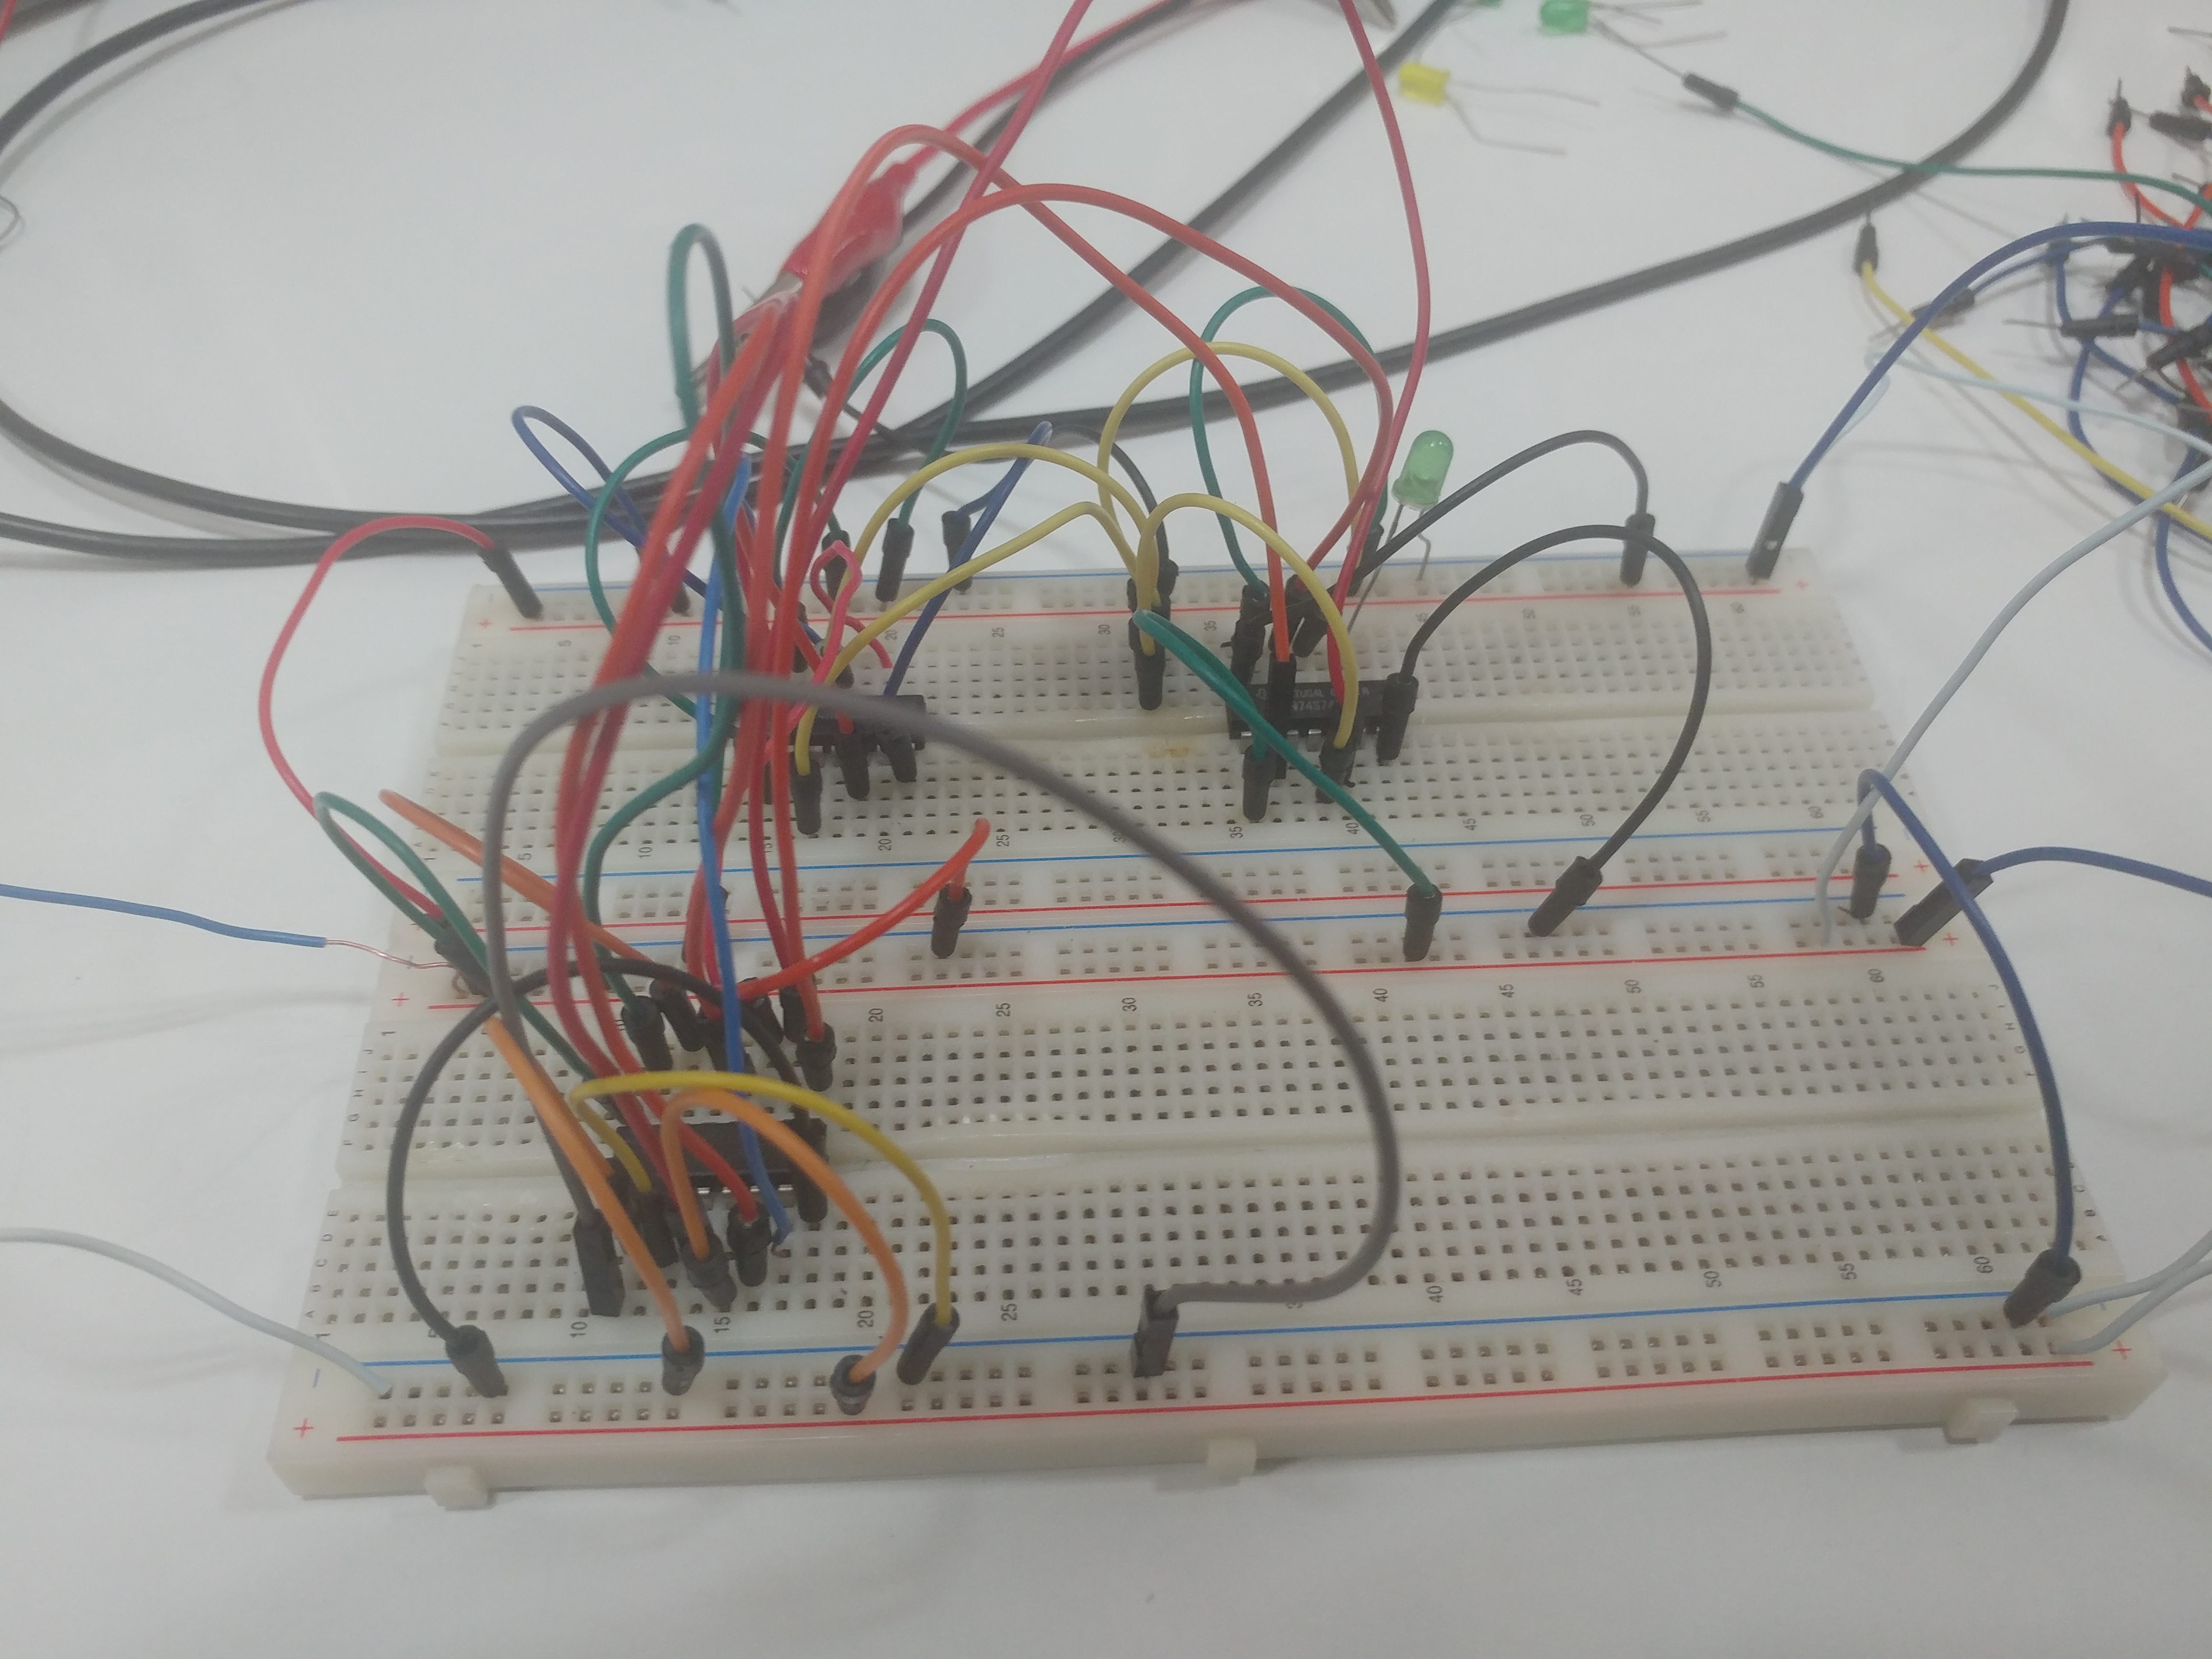
\includegraphics[scale=0.05]{shift_do_tarafe}‎
			\caption{شیفت رجیستر دو طرفه}
		\end{center}
	\end{figure} 
	
	% with 7495
	\begin{figure}[h!]
		\begin{center}
			\includegraphics[scale=0.05]{shifter_with_7495_0}‎
			\caption{مدار بسته شده با تراشه 7495}
		\end{center}
	\end{figure} 
	\begin{figure}[h!]
		\begin{center}
			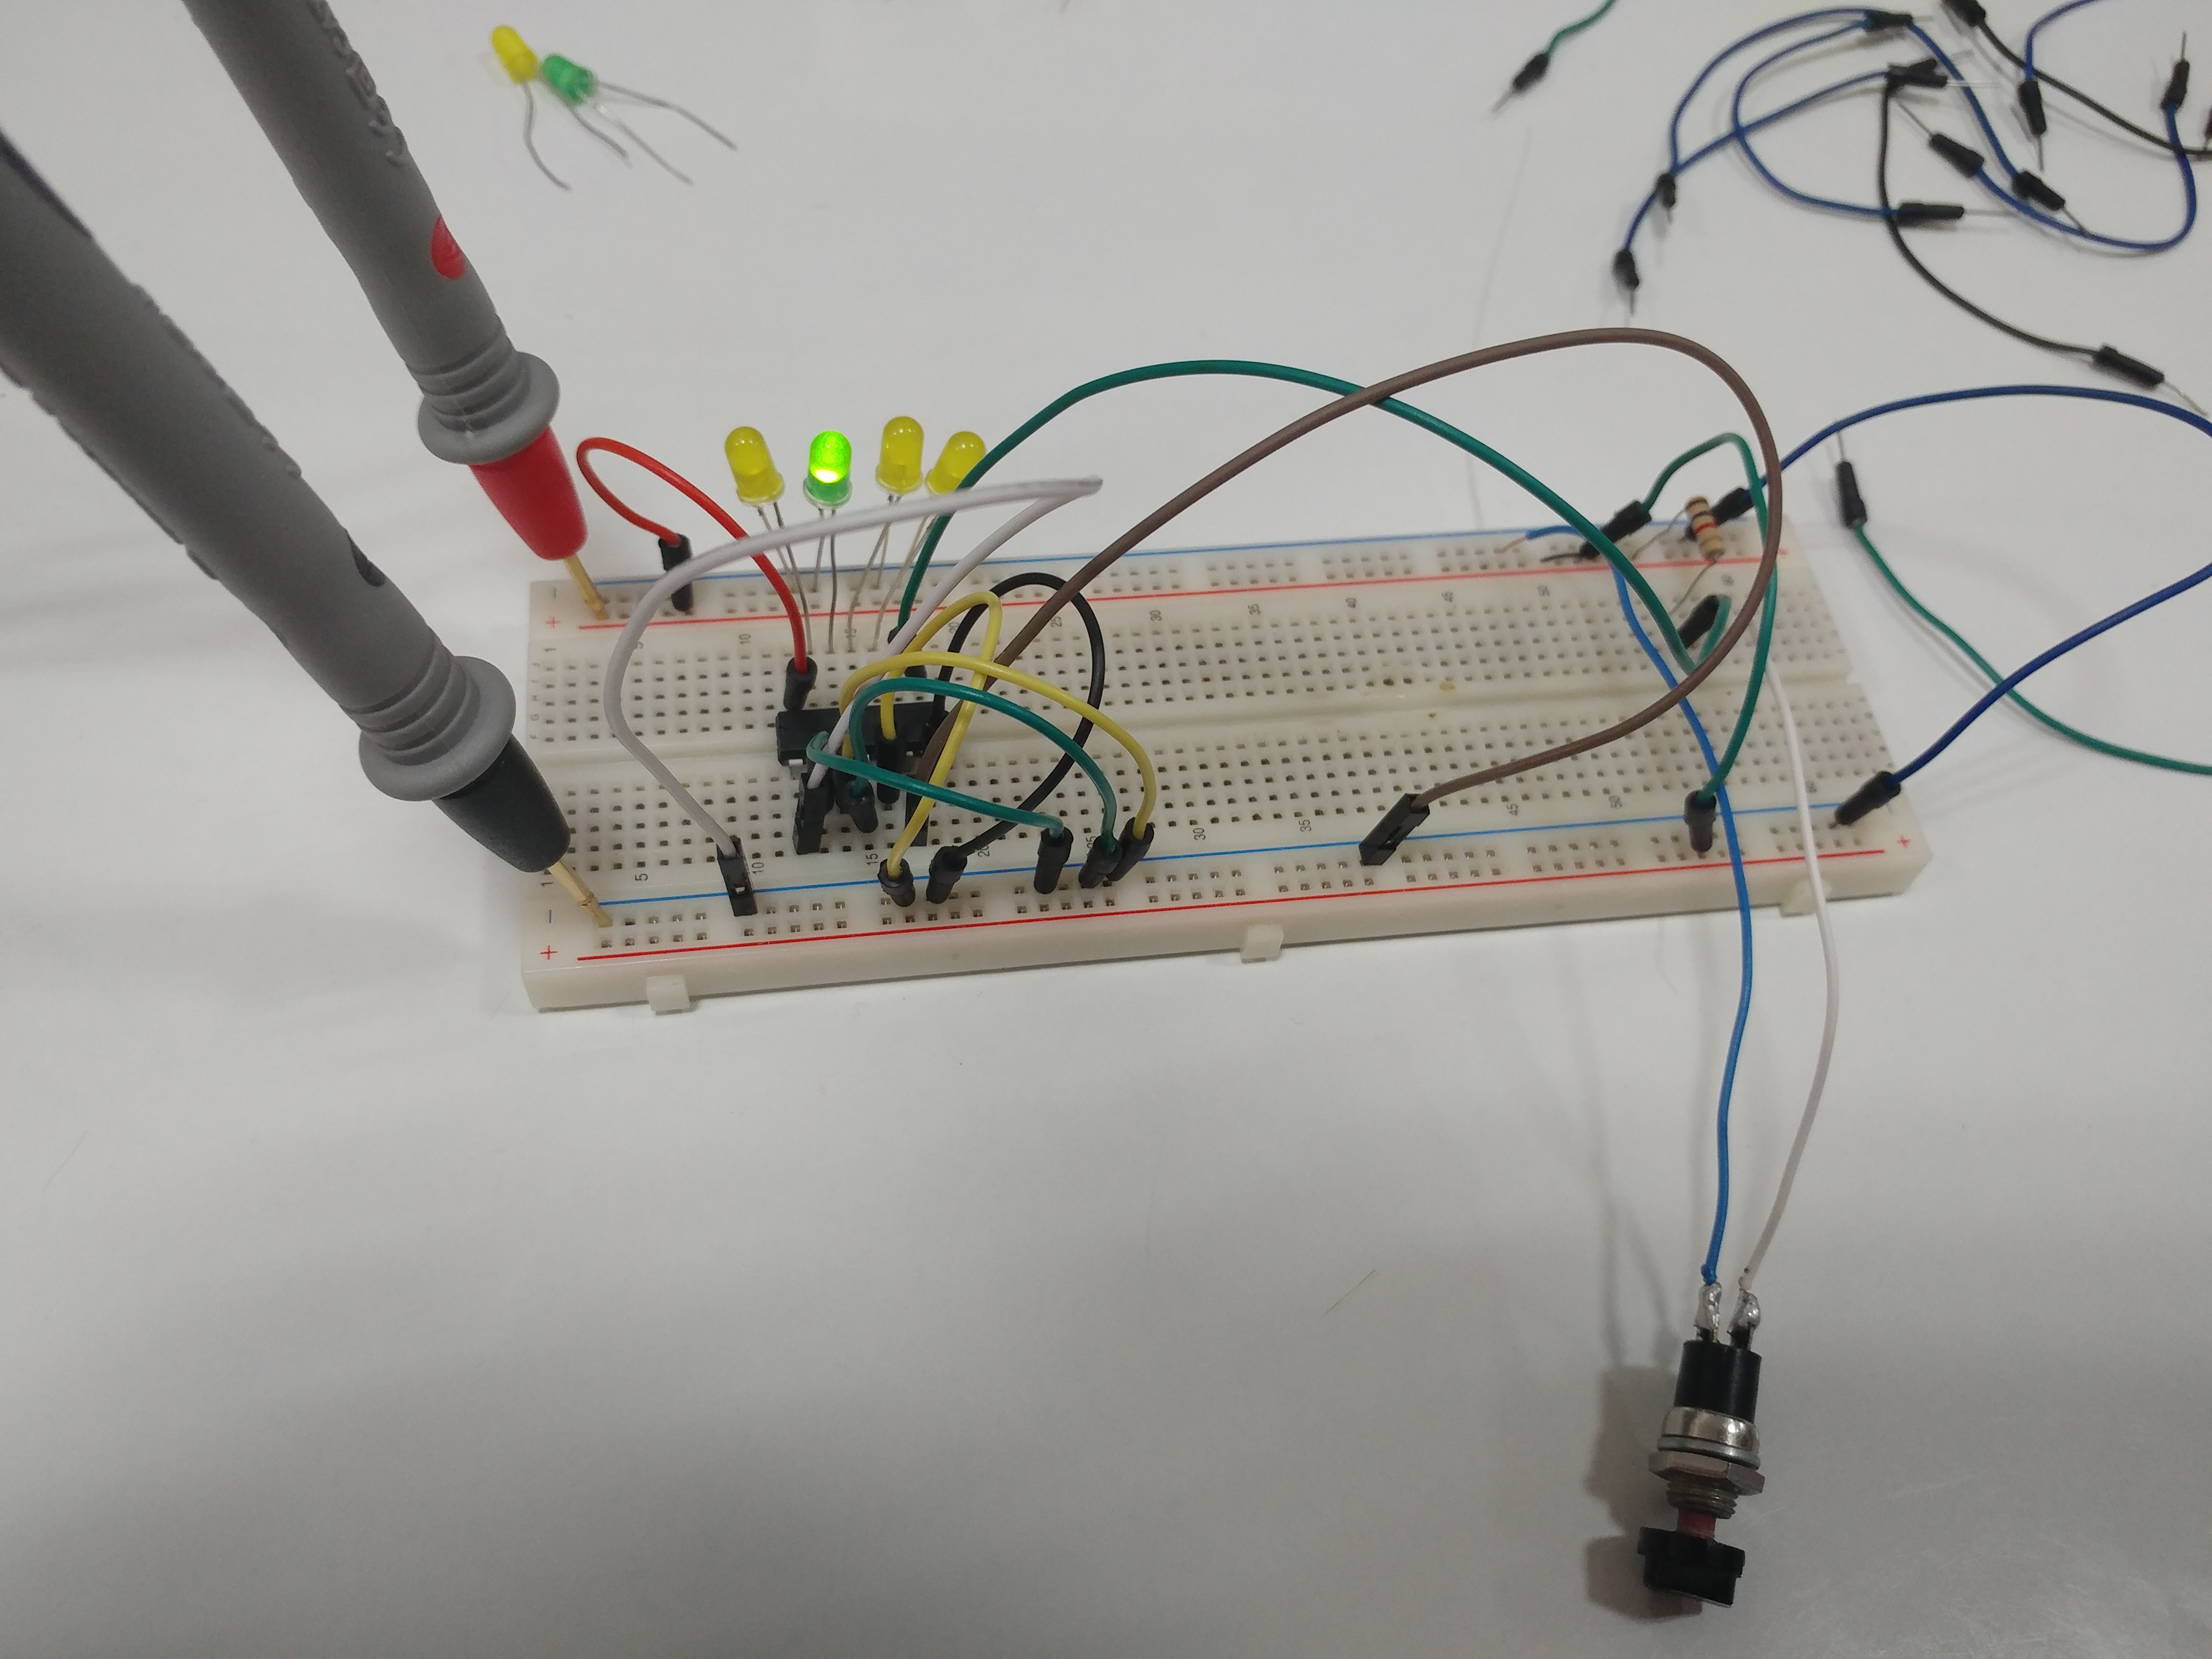
\includegraphics[scale=0.05]{shifter_with_7495_1}‎
			\caption{مدار بسته شده با تراشه 7495}
		\end{center}
	\end{figure} 
	\begin{figure}[h!]
		\begin{center}
			\includegraphics[scale=0.05]{shifter_with_7495_2}‎
			\caption{مدار بسته شده با تراشه 7495}
		\end{center}
	\end{figure} 
	\begin{figure}[h!]
		\begin{center}
			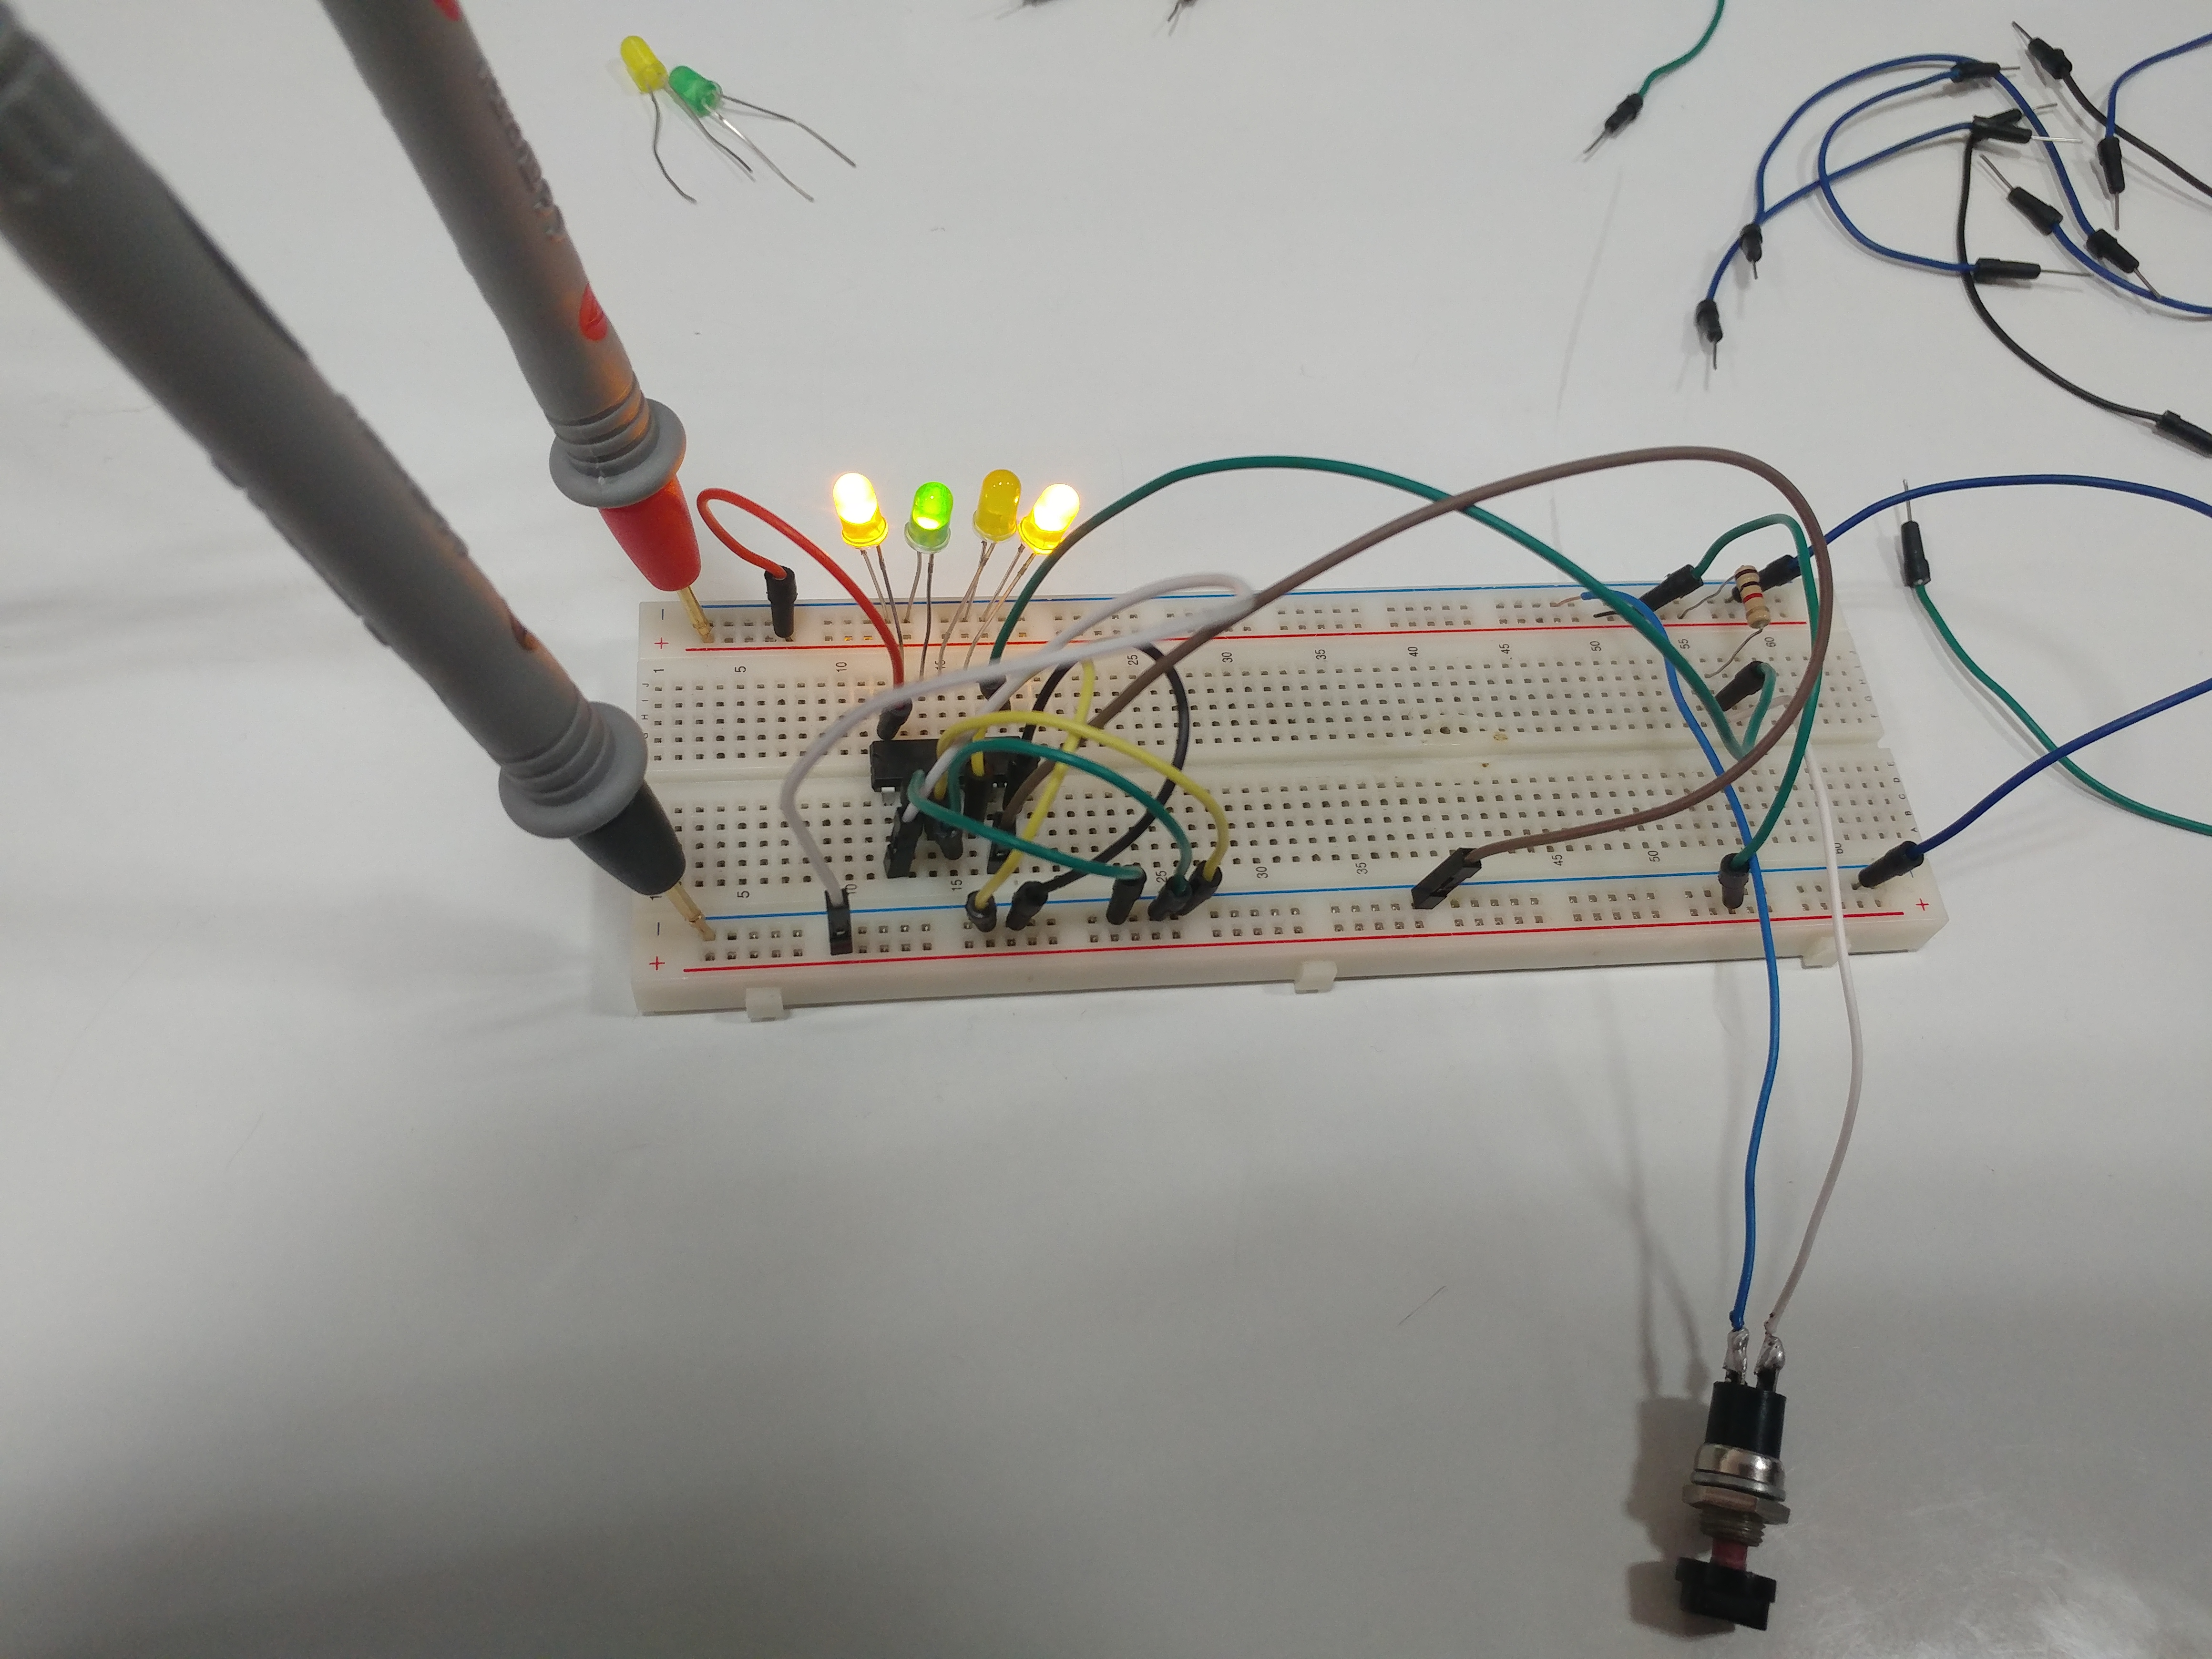
\includegraphics[scale=0.05]{shifter_with_7495_3}‎
			\caption{مدار بسته شده با تراشه 7495}
		\end{center}
	\end{figure} 
	% end of with 7495
	
	\begin{figure}[h!]
		\begin{center}
			\includegraphics[scale=0.6]{johnson_ring_counter}‎
			\caption{شمارنده حلقه 4 بیتی}
		\end{center}
	\end{figure} 
	
	% johnson pics
	\begin{figure}[h!]
		\begin{center}
			\includegraphics[scale=0.05]{j1}‎
			\caption{شمارنده جانسون}
		\end{center}
	\end{figure} 

	\begin{figure}[h!]
		\begin{center}
			\includegraphics[scale=0.05]{j2}‎
			\caption{شمارنده جانسون}
		\end{center}
	\end{figure} 

	\begin{figure}[h!]
		\begin{center}
			\includegraphics[scale=0.05]{j3}‎
			\caption{شمارنده جانسون}
		\end{center}
	\end{figure} 
	
	\begin{figure}[h!]
		\begin{center}
			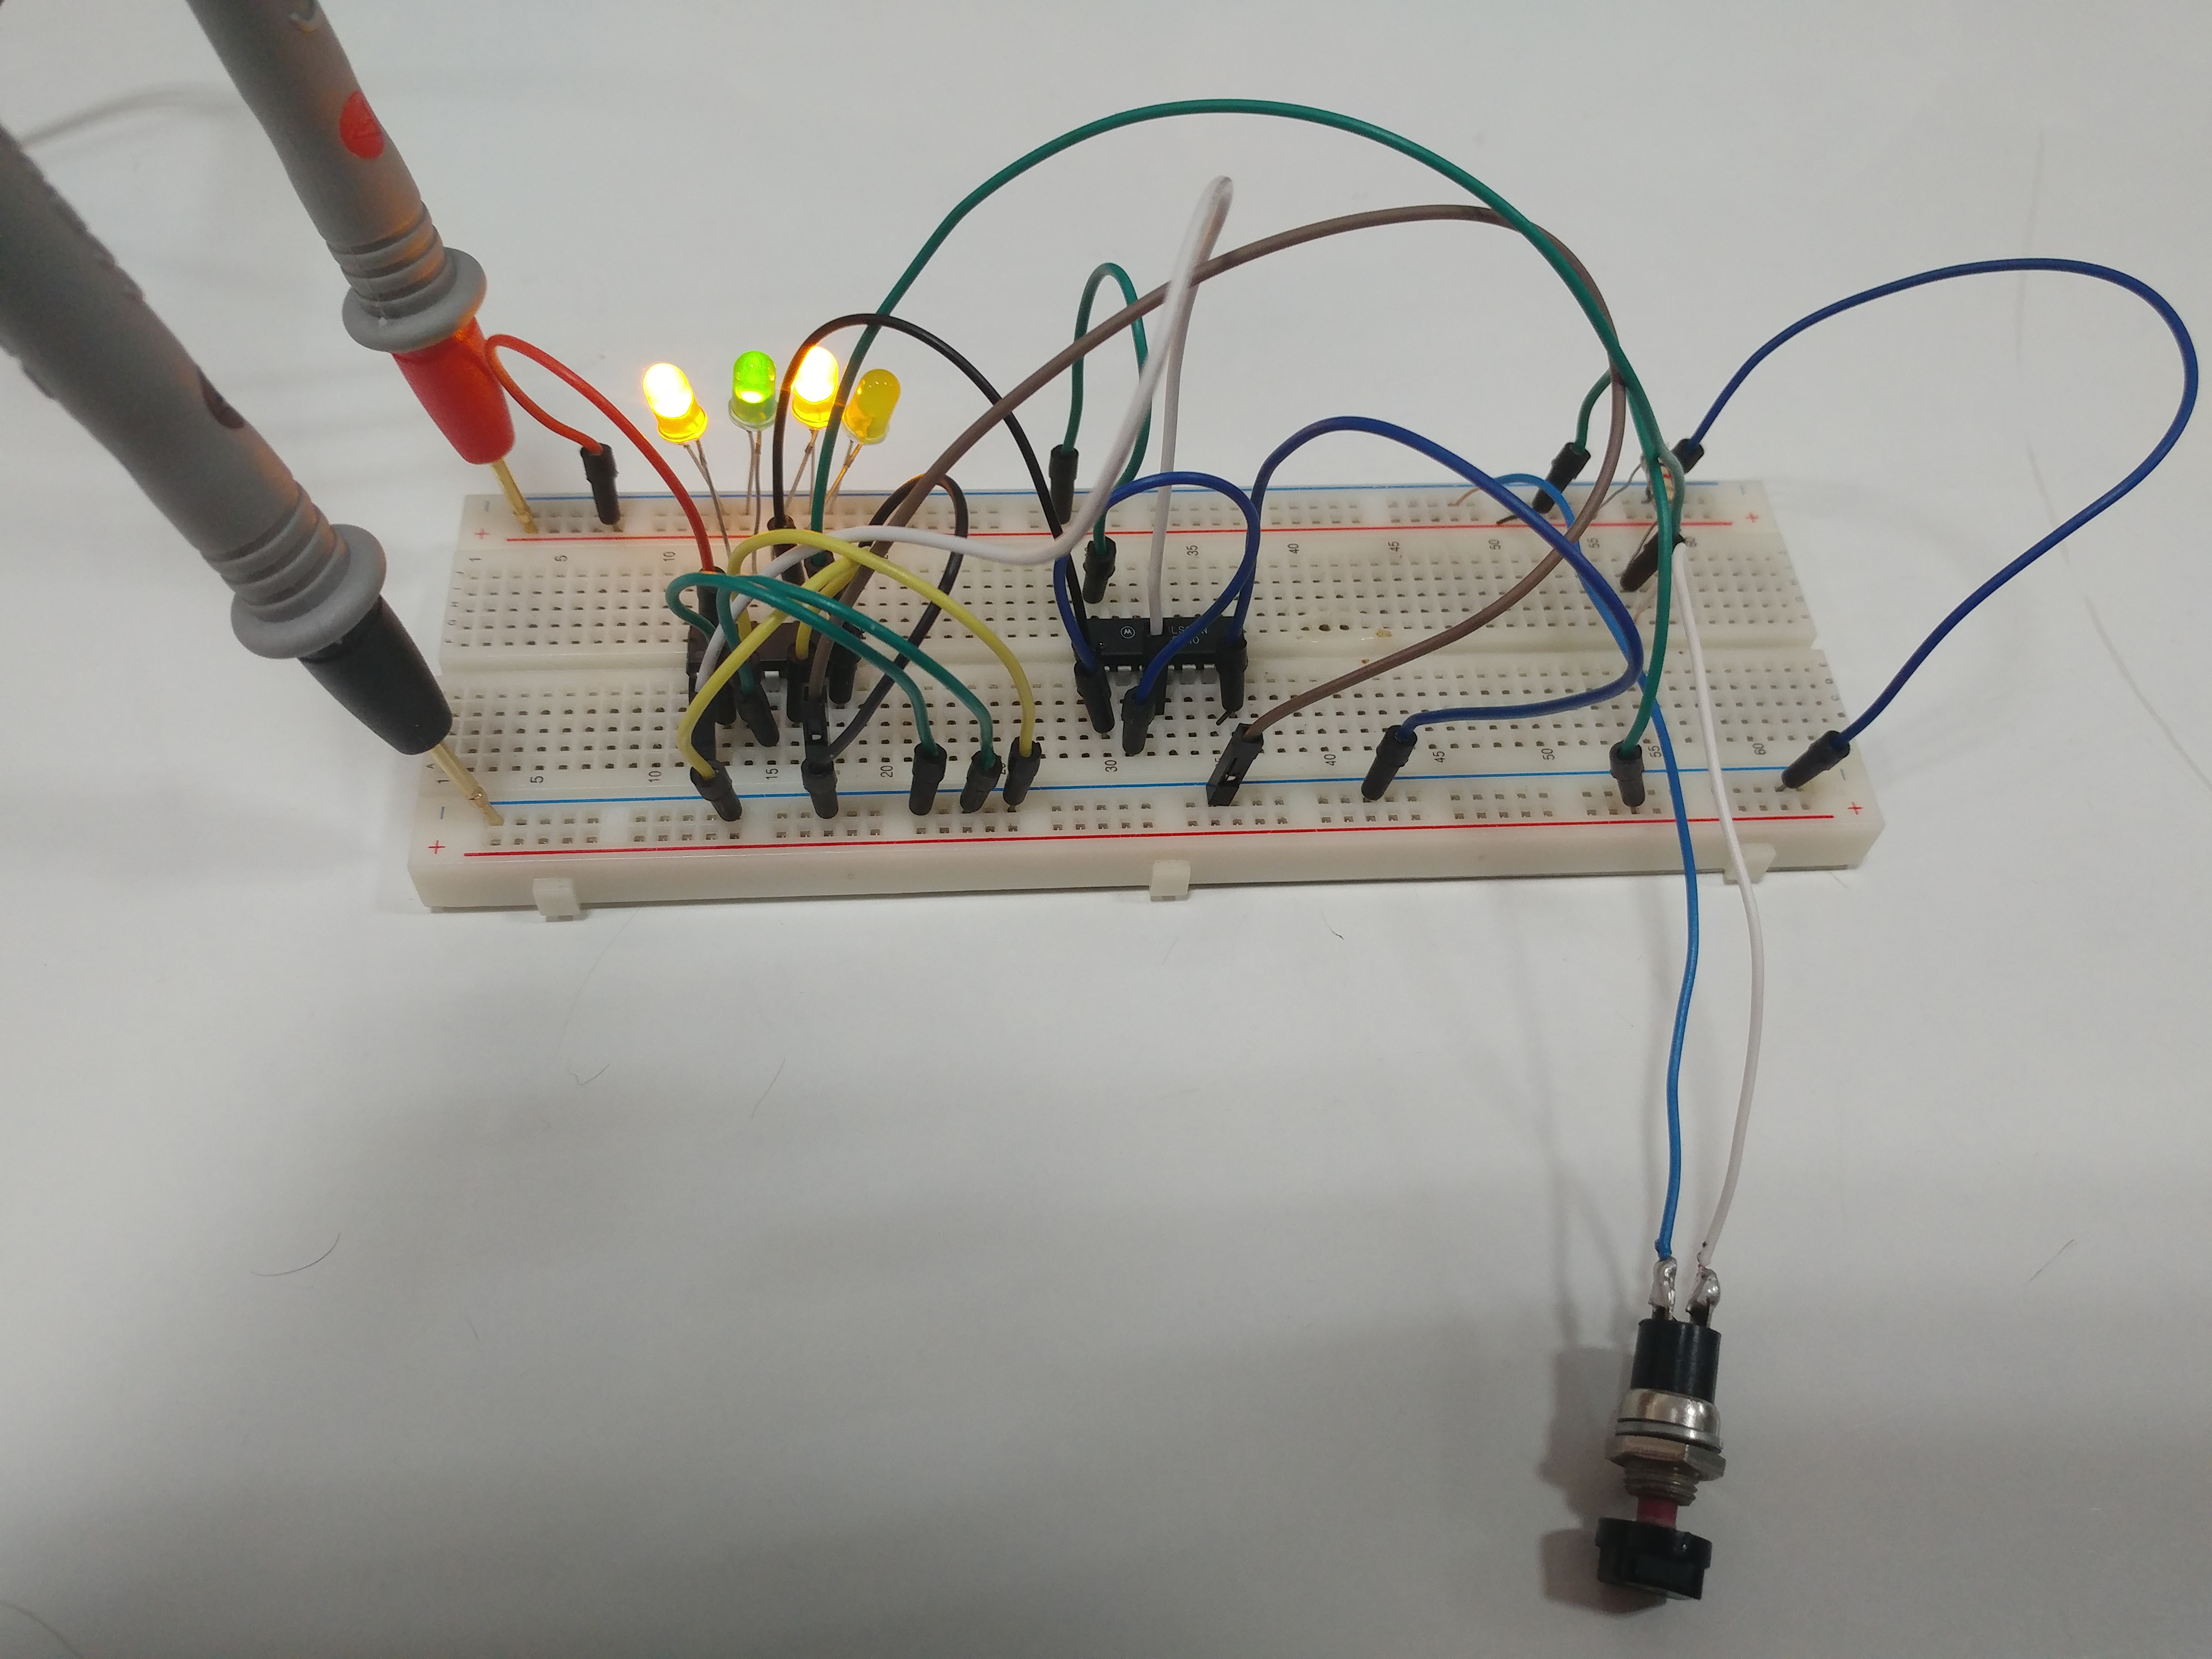
\includegraphics[scale=0.05]{j4}‎
			\caption{شمارنده جانسون}
		\end{center}
	\end{figure} 
	
	\begin{figure}[h!]
		\begin{center}
			\includegraphics[scale=0.05]{j5}‎
			\caption{شمارنده جانسون}
		\end{center}
	\end{figure} 
	
	\begin{figure}[h!]
		\begin{center}
			\includegraphics[scale=0.05]{j6}‎
			\caption{شمارنده جانسون}
		\end{center}
	\end{figure} 
	
	\begin{figure}[h!]
		\begin{center}
			\includegraphics[scale=0.05]{j7}‎
			\caption{شمارنده جانسون}
		\end{center}
	\end{figure} 
	
	\begin{figure}[h!]
		\begin{center}
			\includegraphics[scale=0.05]{j8}‎
			\caption{شمارنده جانسون}
		\end{center}
	\end{figure} 

	% end of johnson pics
	
	\begin{figure}[h!]
		\begin{center}
			\includegraphics[scale=0.75]{7495_connection_diagram}‎
			\caption{تراشه 7495}
		\end{center}
	\end{figure} 
	
	\begin{figure}[h!]
		\begin{center}
			\includegraphics[scale=0.6]{7495_function_table}‎
			\caption{ جدول عملکردی تراشه 7495}
		\end{center}
	\end{figure} 
	
\end{document}









